\documentclass{report}
\usepackage{hyperref}
\usepackage{amsmath}
\usepackage{array}
\usepackage{longtable}
\usepackage[margin=1in]{geometry}
\usepackage{graphicx}

\graphicspath{{./images/}{../../out/docs/report/diagrams}}

\newcolumntype{R}[1]{>{\raggedleft\arraybackslash}p{#1}}
\newcolumntype{L}[1]{>{\raggedright\arraybackslash}p{#1}}

\title{Coding Languages and Salary}
\author{Thomas Kwashnak}

\begin{document}

\maketitle

\tableofcontents

\newpage

\chapter{Introduction}
In the grand scheme of history, coding has been around for very little time. In that time, however, the coding industry has changed countless times as new languages and frameworks pop up, and others die off. Now, there are countless programming langauges and frameworks that people use for various tasks. Some excel at writing low-level and efficient code used in operating systems, while others sacrifice efficiency for ease of use.

Coding has turned into an industry. Multiple industries, in fact, that use programming languages to automate certain tasks, calculate results, create entertainment, and many other applications. Programming has now become one of the many in-demand jobs in the world. However, for those who may not be in the know, seeing the countless programming languages might be intimidating. It's wildly debated about which languages earn the most money.

The purpose of this paper is to explore these relationships, creating a model that describes which languages correlate to an increase in salary. The goal is that by the end of this project, we will have better guidance as to what languages are most worth it to learn. In other words, we are trying to figure out how to approach choosing languages to learn.

\chapter{Data}

\section{What data?}

It can be argued that Stack Overflow has been a vital source of information for the programming industry. Searching up almost any coding-related question will send you to a stackoverflow post asking the same or similar question. StackOverflow has become a hub for programmers to learn from the years of questions asked.

Taking advantage of the traffic that StackOverflow gets, every year they ask users to fill out a survey about their experiences with coding. The questions range from asking their education status to what frameworks they work with. Once they've compiled it together, they create a webpage that summarizes the data they find.\footnote{The results for the year 2022: \href{https://survey.stackoverflow.co/2022/}{survey.stackoverflow.co/2022/}}

In addition to publishing their findings, they also offer an anonymized version of the dataset for download. In this paper, we will be using this dataset from the year 2022\footnote{You can download and explore the data: \href{https://insights.stackoverflow.com/survey/}{insights.stackoverflow.com/survey/}} as it includes many of the variables we need.

\section{What's in the Data Set}

The dataset that we will be using has 79 columns of data, many that can be parsed out into many more. Below are the columns of data that are most interesting to our question, including the direct variables and controls that we may need to set.

\begin{longtable}{| p{0.3\textwidth} | p{0.7\textwidth} |}
\hline
\textbf{Employment} & Whether the individual is employed full or part time, is an independant contractor, or a full or part-time student \\ \hline
\textbf{EdLevel} & The level of education that the individual has completed, whether it's primary school, associates, undergraduate, etc. \\ \hline
\textbf{YearsCode}& The number of years that the individual has been programming for. \\ \hline
\textbf{YearsCodePro} & The number of years that the individual has been professionally programming for. \\ \hline
\textbf{DevType} & The types of developer that the individual falls under. This is a multi-selected list, so the individual may indicate multiple developer types. The developer types range from front end, back end, data engineer, and other similar roles. \\ \hline
\textbf{Country} & The country that the individual lives in \\ \hline
\textbf{Currency} & The currency that the individual uses \\ \hline
\textbf{CompTotal} & The total compensation that the individual recieves \\ \hline
\textbf{CompFreq} & The frequency that the individual recieves their compensation for working. \\ \hline
\textbf{WorkExp} & The number of years of work experience the individual has had \\ \hline
\textbf{LanguageHaveWorkedWith} & A multi-select list of languages that the individual has worked with in the last year. \\ \hline
\textbf{LanguageWantToWorkWith} & A multi-select list of languages that the individual wants to work with in the next year \\ \hline
\textbf{ConvertedCompYearly} & While this variable isn't well documented, it appears to be a converted yearly compensation for each individual. There is no thorough documentation that describes the reasoning behind which entries have this populated and which do not, but there are enough values to use this effectively \\ \hline
\end{longtable}

While the dataset does contain many more variables, and you are welcome to explore it on your own, these are the variables that we will be primarily using in our analysis.

\section{Filtering Data}

The dataset is pretty large. Since it was from an open poll, we aren't able to really trust each and every reported value. However, one of the values found in the dataset seem to be only listed for select entries, and not the outliers. We will be using that to filter out any excess data. Additionally, we will be filtering to only individuals within the United States. To keep the data tame, I've also filtered out any entries of yearly compensation over $\$1,000,000$.

I've also had to remove some of the possible values from variables. Most notably, in order to avoid multi-collinearity I removed the values in the Education variable that pertained towards current education. That is, the Education variables now only consist of higher-education and not partial or lower education.

\section{Data Statistics}

Below are some interesting statistics that we should keep in mind, since they might have some impact on how the analysis we extract is.

\vspace{0.5in}

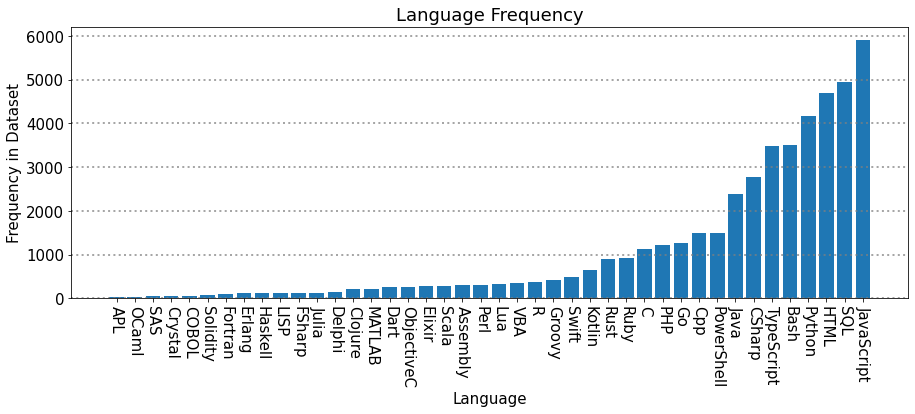
\includegraphics[width=0.9\linewidth]{frequencyLanguage.png}

\vspace{0.5in}

The frequency of each language gives us a gauge of what the standard deviations we expect each language to have. Specifically, languages that have fewer entries, such as APL, may not be able to be accurately represented in our models, due to the lack of data.

\vspace{0.5in}

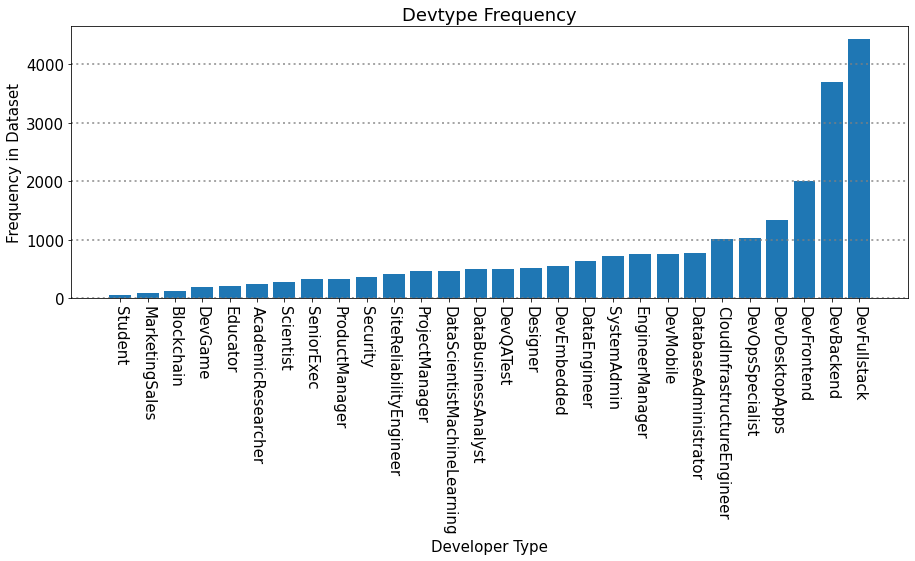
\includegraphics[width=0.9\linewidth]{frequencyDevtype.png}

\vspace{0.5in}

The frequency of the developer types gives us an idea of what our dataset is comprised of. From the graph above, we can see that our data seems to be mostly Front, Back, and Full-stack developers. This makes sense because StackOverflow gets the most traffic from these sources. This means that our results will be more geared towards those types of developments.

Many of the other developer types are also partially included in the full-stack scope, but were listed separately.

\vspace{0.5in}

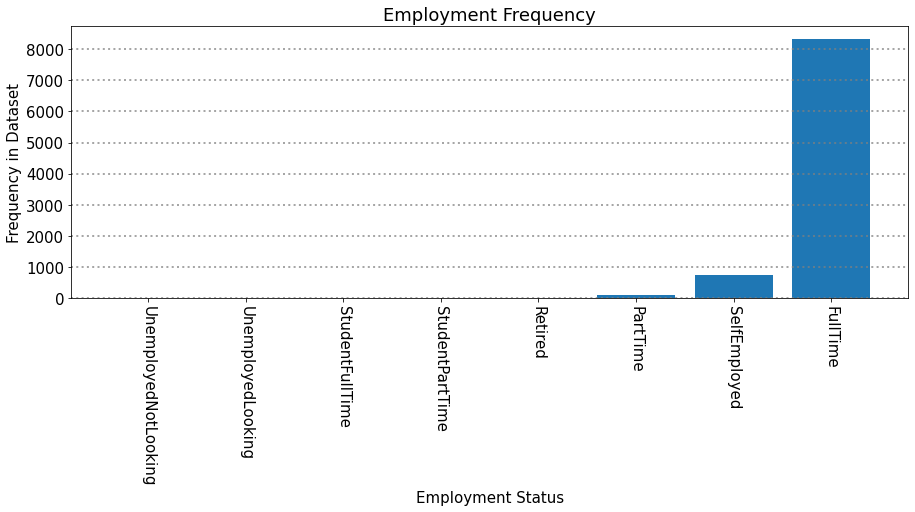
\includegraphics[width=0.9\linewidth]{frequencyEmployment.png}

\vspace{0.5in}

As it appears in the visualization, it appears that our dataset is comprised of mostly full-time, part-time, and self-employed developers. Because of this, we can ignore the other categories.

\vspace{0.5in}

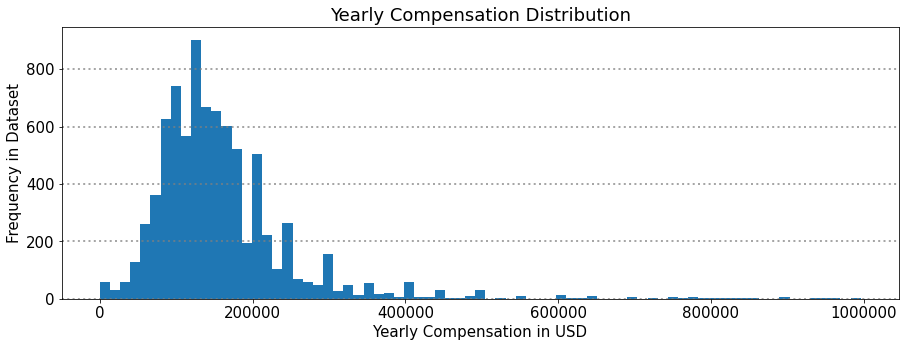
\includegraphics[width=0.9\linewidth]{frequencyConvertedCompYearly.png}

\vspace{0.5in}

As seen here, the distribution seems to mainly hover around $\$100,000$ to $\$200,000$ with some outliers both higher and lower. One of the mistakes I made while building the model was forgetting to restrict the compensation down to at most $\$1,000,000$. Now that the range seems reasonable, the data should mostly be accurate and usable.


\chapter{Data Analysis}

\section{The Model}

The model used to draw conclusions is tasked to find relationships between coding languages and salary. I controlled for various variables, including the developer type, years professionally programming, and employment status.

\subsection{Causality Analysis}

\includegraphics[width=0.95\linewidth]{model.png}

The graph above indicates the causality graph used for building the model. As indicated, the blue nodes represent the relationship I want to focus on. In my instance, that is the programming languages and salary. The other nodes are other aspects that relate programming languages and salary together. Nodes in green indicate aspects that I will be controlling in my model.

\subsection{Model Equation}

The model I have decided to use is as follows.

$$\log(\text{Salary}) = \beta_0 + \beta_1 \text{Years Work} + \beta_2 \sum_h{\beta_h \text{Education}} + \sum_i{\beta_i \text{Programming Languages}} + \sum_j{\beta_j \text{Dev Type}}$$

The first point to notice about the model equation is that I've used summations. The reason I've used summations is because there are far too many variables in each `category' to include it in the summary. Most of these variables are binary values.The only non-binary value is the number of years that an individual has worked.

Because we are using log base 10, the interpretation of the coefficients are different. For binary coefficients such as those found in the Education, Developer Type, and Programming Language sections, the coefficient means that individuals with that property have a $\beta \cdot 100\%$ change in pay. For example, if the coefficient of having a Masters degree is $0.15$, then having a masters degree increases your salary by $15\%$.

However, for the Years Working coefficient, the interpretation is different. The coefficient on Years Working indicates that for every year you work, your salary goes up $\beta \cdot 100\%$. For example, if the coefficient on Years Working is $0.04$, and you have worked 5 years, the effect of your work experience is that your salary is $20\%$ higher than someone who has no work experience.


\subsection{Coefficient Values}

The complete model's coefficient values are listed in a table below. Don't try to interpret this, there are graphs after the table that visualize the important features of the model.

\begin{longtable}{|R{0.4\linewidth}|R{0.3\linewidth}|R{0.3\linewidth}|}
  \hline
  \textbf{Coefficient} & \textbf{Coef.} & \textbf{Std.Err.} \\

  \hline
  $Intercept$ & $5.018561975617827$ & $0.014839004672467472$\\
  \hline
  $APL$ & $-0.08449616172936489$ & $0.07031461604245251$\\
  \hline
  $Assembly$ & $0.016543407577874203$ & $0.023222811832528233$\\
  \hline
  $Bash$ & $0.022502299799285364$ & $0.008126254562779637$\\
  \hline
  $C$ & $-0.004627316713939622$ & $0.014173655368536292$\\
  \hline
  $CSharp$ & $-0.012588890609753975$ & $0.009085160939920714$\\
  \hline
  $Cpp$ & $0.0013302181178897199$ & $0.011912263426960995$\\
  \hline
  $COBOL$ & $-0.05980366511464108$ & $0.045879491473421935$\\
  \hline
  $Clojure$ & $0.05637302678016759$ & $0.024627811466780104$\\
  \hline
  $Crystal$ & $-0.07234531945106182$ & $0.04327405939866166$\\
  \hline
  $Dart$ & $-0.00917484299525742$ & $0.02189492641781949$\\
  \hline
  $Delphi$ & $-0.0693890922496736$ & $0.03586179425005313$\\
  \hline
  $Elixir$ & $0.02210851459062957$ & $0.024672292276064385$\\
  \hline
  $Erlang$ & $0.024650132224725452$ & $0.03868532133487006$\\
  \hline
  $FSharp$ & $0.003168089676544944$ & $0.029181773275287513$\\
  \hline
  $Fortran$ & $-0.048333855664798586$ & $0.04105847118866435$\\
  \hline
  $Go$ & $0.05335781525928454$ & $0.010977386023936398$\\
  \hline
  $Groovy$ & $0.001605072885167258$ & $0.01751638180083541$\\
  \hline
  $HTML$ & $-0.028033485222218463$ & $0.009103744949128282$\\
  \hline
  $Haskell$ & $0.008404301828283167$ & $0.03192838464217453$\\
  \hline
  $Java$ & $0.01937787833703439$ & $0.008896786629214502$\\
  \hline
  $JavaScript$ & $-0.0027372986809501565$ & $0.010224848456465157$\\
  \hline
  $Julia$ & $-0.015498841494914456$ & $0.03534525669461834$\\
  \hline
  $Kotlin$ & $0.01054821064480578$ & $0.014670749859060759$\\
  \hline
  $LISP$ & $-0.017472537118401965$ & $0.03295181888669319$\\
  \hline
  $Lua$ & $-0.030831776743935557$ & $0.020575394583910264$\\
  \hline
  $MATLAB$ & $-0.021213647704870414$ & $0.025002721413724522$\\
  \hline
  $OCaml$ & $0.05015895016782079$ & $0.06719487153425305$\\
  \hline
  $ObjectiveC$ & $0.07222513095095705$ & $0.02481404571568205$\\
  \hline
  $PHP$ & $-0.0544365718219032$ & $0.011143311982348787$\\
  \hline
  $Perl$ & $-0.006106768354959213$ & $0.020625334173556737$\\
  \hline
  $PowerShell$ & $-0.014147923875509484$ & $0.010386913376311395$\\
  \hline
  $Python$ & $0.002687297090511978$ & $0.008151030909738132$\\
  \hline
  $R$ & $-0.030262557602700052$ & $0.020931196440234025$\\
  \hline
  $Ruby$ & $0.028956172482974392$ & $0.011908465402361249$\\
  \hline
  $Rust$ & $0.018212887227691488$ & $0.012870849262221455$\\
  \hline
  $SAS$ & $-0.013234736089247523$ & $0.052013262317076876$\\
  \hline
  $SQL$ & $-0.00849666228036599$ & $0.008284963162838334$\\
  \hline
  $Scala$ & $0.025163815292020053$ & $0.021331433168606025$\\
  \hline
  $Solidity$ & $-0.0427805336085689$ & $0.0389795415592104$\\
  \hline
  $Swift$ & $0.004164081839166639$ & $0.01896091451038442$\\
  \hline
  $TypeScript$ & $0.04359114908560244$ & $0.008403383876866784$\\
  \hline
  $VBA$ & $-0.011001469110574008$ & $0.019243503113297276$\\
  \hline
  $AcademicResearcher$ & $-0.12871697651357228$ & $0.02730337888145829$\\
  \hline
  $Blockchain$ & $0.06578162262406473$ & $0.03372859156753758$\\
  \hline
  $CloudInfrastructureEngineer$ & $0.05196419915888793$ & $0.012553737347643696$\\
  \hline
  $DataBusinessAnalyst$ & $-0.039286887324647385$ & $0.01728960385438497$\\
  \hline
  $DataScientistMachineLearning$ & $0.023357961295502674$ & $0.018307419762844942$\\
  \hline
  $DatabaseAdministrator$ & $-0.027028506649393783$ & $0.014987678291949746$\\
  \hline
  $Designer$ & $-0.04223410477458675$ & $0.01651835731226557$\\
  \hline
  $DevOpsSpecialist$ & $-0.001873958169947676$ & $0.012705858826887234$\\
  \hline
  $DevQATest$ & $-0.03476863560289306$ & $0.0159755981159479$\\
  \hline
  $DevBackend$ & $0.04031953686858543$ & $0.008087778525870913$\\
  \hline
  $DevDesktopApps$ & $-0.004829218147118508$ & $0.01085656243606461$\\
  \hline
  $DevEmbedded$ & $-0.010143810224208738$ & $0.016861477544157503$\\
  \hline
  $DevFrontend$ & $-0.0168633431055481$ & $0.009973702591350013$\\
  \hline
  $DevFullstack$ & $-0.0034240279451892147$ & $0.008468785646300603$\\
  \hline
  $DevGame$ & $-0.021734376551434786$ & $0.025061044914121103$\\
  \hline
  $DevMobile$ & $0.0040507442759937715$ & $0.014740447453515668$\\
  \hline
  $Educator$ & $-0.059312619088188856$ & $0.026376953428444504$\\
  \hline
  $DataEngineer$ & $0.03490855530981987$ & $0.014714236436138586$\\
  \hline
  $SiteReliabilityEngineer$ & $0.04767241459003019$ & $0.017807501780216103$\\
  \hline
  $EngineerManager$ & $0.06223673153071544$ & $0.012756460781307929$\\
  \hline
  $MarketingSales$ & $-0.03356290987567101$ & $0.04164521180502019$\\
  \hline
  $ProductManager$ & $0.04436042786336988$ & $0.021278861228822374$\\
  \hline
  $ProjectManager$ & $-0.025467515919178063$ & $0.018275603212142864$\\
  \hline
  $Scientist$ & $-0.029241818484850468$ & $0.026753834531422153$\\
  \hline
  $Security$ & $0.0054076517835031646$ & $0.01889144747180604$\\
  \hline
  $SeniorExec$ & $0.07737027618438086$ & $0.02021619055971414$\\
  \hline
  $Student$ & $-0.12365568225571719$ & $0.04483903654046471$\\
  \hline
  $SystemAdmin$ & $-0.06452130456738468$ & $0.01494683899507614$\\
  \hline
  $AssociatesDegree$ & $-0.05102391960598193$ & $0.019700448959642704$\\
  \hline
  $BachelorsDegree$ & $0.025741588647834768$ & $0.01081393797362146$\\
  \hline
  $MastersDegree$ & $0.06254927197146623$ & $0.012988286347159678$\\
  \hline
  $DoctoralDegree$ & $0.12807670365517893$ & $0.0248851638560115$\\
  \hline
  $ProfessionalDegree$ & $0.0892062562999687$ & $0.04616626957254842$\\
  \hline
  $WorkExp$ & $0.00479688874852874$ & $0.0003893979526814846$ \\
  \hline
\end{longtable}

\newpage
\section{Model Analysis}
The table above does a great job of telling you the details, however it doesn't give us anything that we can easily interpret. That's where graphs can come in to help!

\vspace{0.5in}

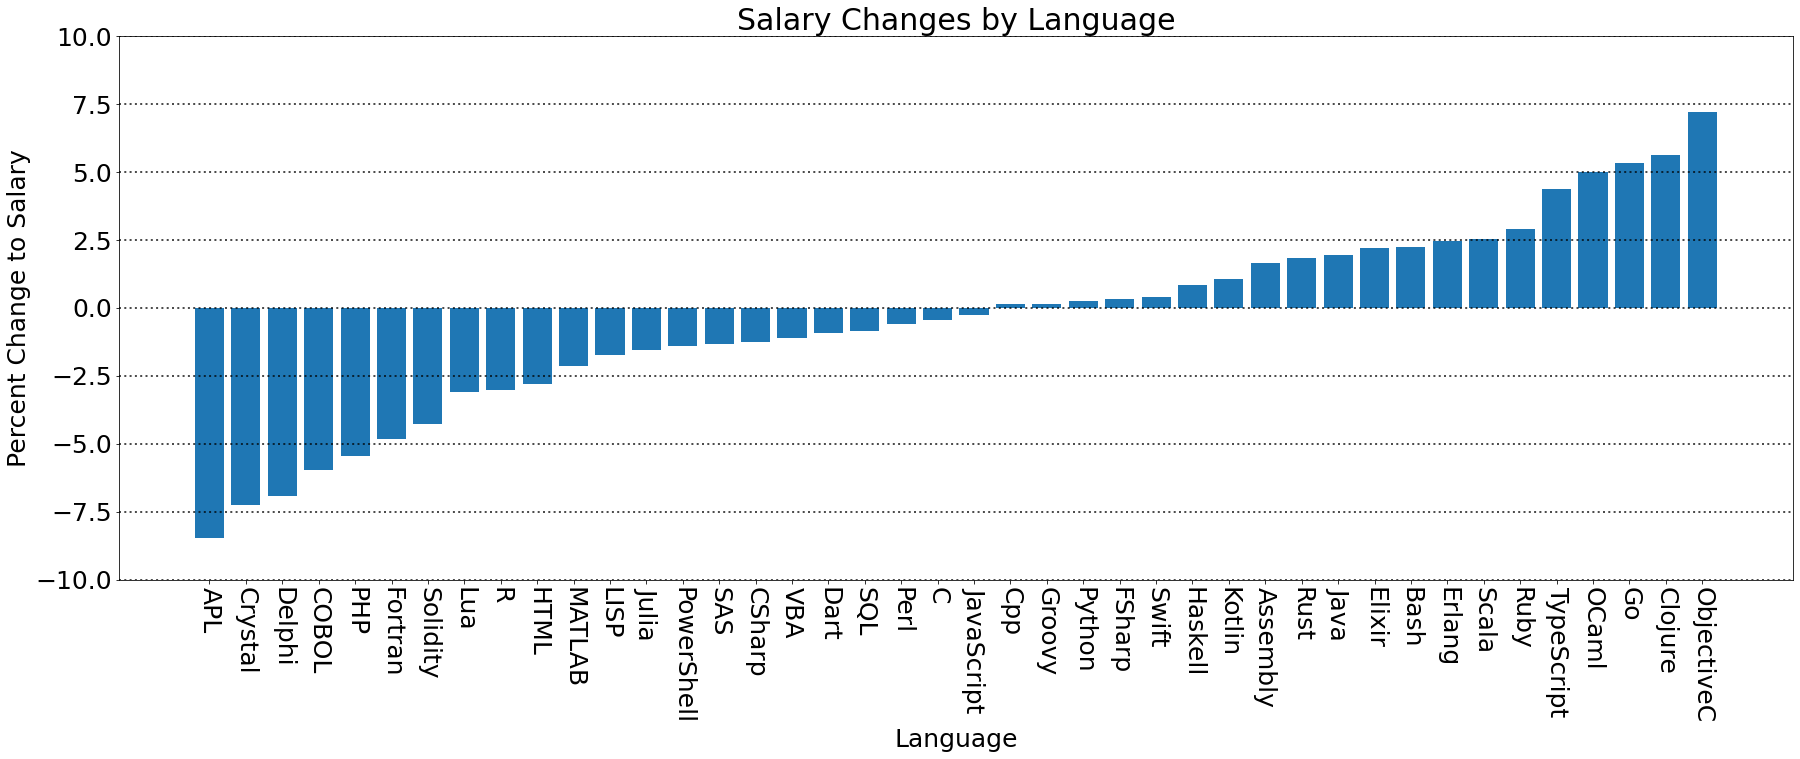
\includegraphics[width=0.95\linewidth]{coefficients_language.png}

\vspace{0.5in}

This graph shows us the distribution of the coefficients on langauges. In short, it gives us an ordered visual on different languages and their effects on salary. Languages on the right side of the graph increase the salary of those who work with them, and languages on the left decrease the salary. The `average', or the base salary of any individual, is not the average salary of a developer.

An interesting feature I noticed is that languages that are used most often, or languages I knew to be used a lot, find themselves in the center. Perhaps this is because those languages somewhat become the 'baseline' that the regression bases off of. That makes sense as the languages at both extremes are languages more specific towards a particular field.

While building the model, I ran into many issues with multi-collinearity. The most substantial were values in Education that fit elsewhere. In the raw dataset, it was possible to put in `SomeCollege' or `PrimarySchool'. However, that often applied to students who also put `Student' in the Developer Type. In order to avoid this, I simply removed the `SomeCollege', `PrimarySchool', and `SecondarySchool' values from the model.

Another graph that gives us insights is looking at the standard deviation of each variable. Basically, take the graph above, make everything positive, and then divide each variable by its standard devation. Thats how we get this:


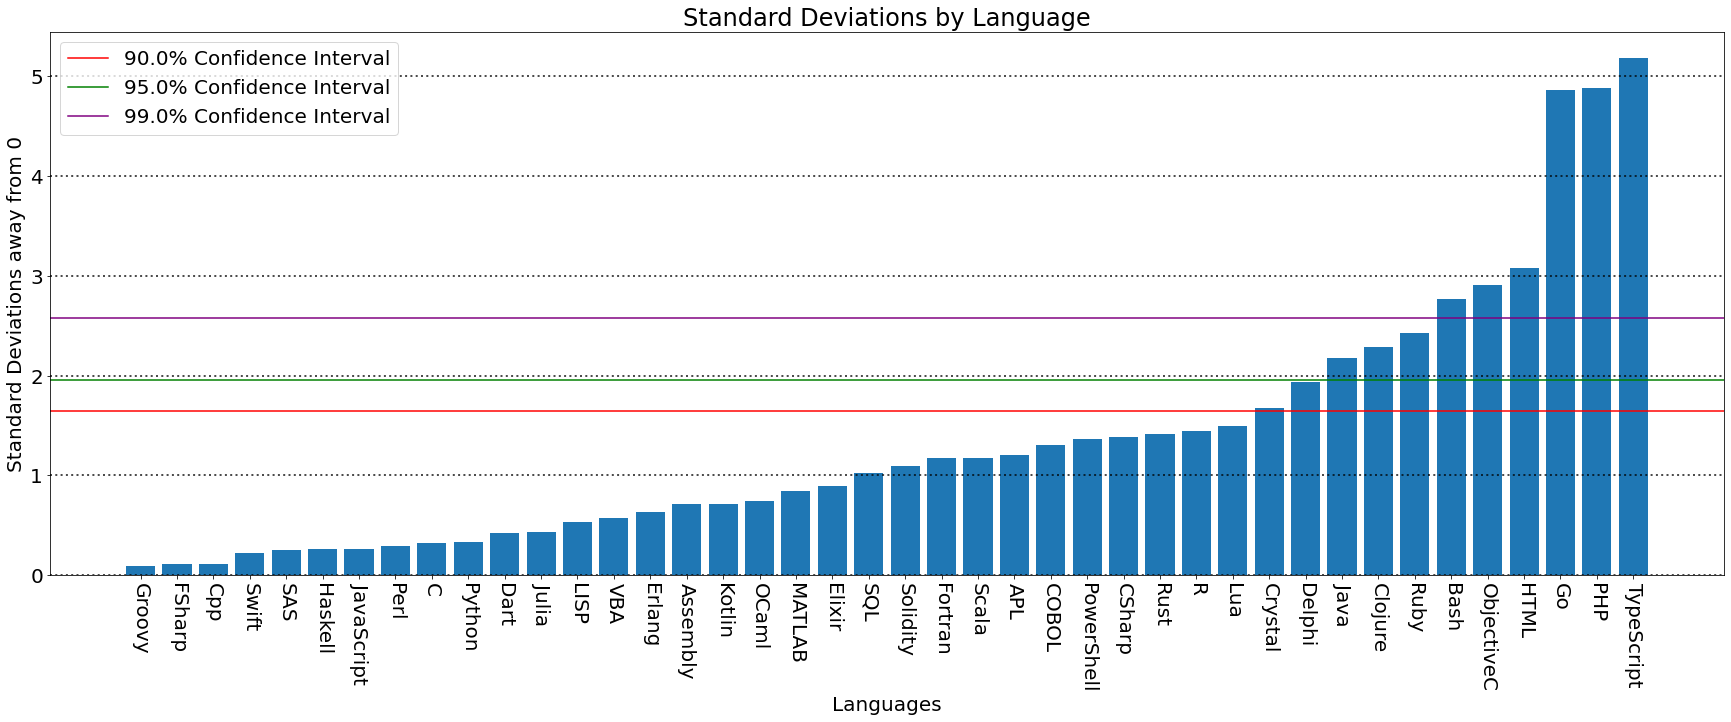
\includegraphics[width=0.95\linewidth]{standarddeviations_language.png}

\vspace{0.5in}

The colored lines on the graph indicate the threshold points for the corresponding confidence intervals. If a coefficient is higher than that threshold, it is found to be statistically significant in the model. While this doesn't give us information about all of the languages, it does give us some insight as to what languages make the difference. If I was to base my conclusions off of the model alone, this would tell me that only a few languages have significant impact on salary, being Typescript, PHP, Go, HTML, ObjectiveC,
and Bash.

Looking at the overall results, there are some langauges I didn't expect to see in their spots. For example, HTML has a very interesting position. In all of my prior work until I got to this model, HTML has always had a negative coefficient. I believe this is because most work in HTML is done by programmers who are entry-level or junior developers. Once someone gets to senior level, most of their work is more advanced, and typically doesn't include HTML work.

Overall, my hypothesis that there are some languages that result in a higher salary than others is generally supported. It does appear that there is indeed a relationship. The relationship itself may not be accurate, as I may need to get more data in order to fully investigate, but the idea is still there.

\chapter{Conclusion}

I think the most factual thing that I can conclude from this analysis is that there is indeed a relationship between languages used and salary. However, the model I built may not have enough data to properly identify the true relationship.

However, some patterns in the model may point us in the right direction. For example, most of the multi-purpose languages fall around the average. That is, picking up another multi-use language isn't going to change someone's salary much. However, as you go towards both extremes, you reach some of the more peculiar and specific languages. For example, Objective-C. Because these languages have a very specific application, they tend to be paid either significantly more or significantly less than average.

Many times people suggest picking up Python, Javascript, HTML, and other languages that are more multi-purpose. Firstly, it's easier to learn something that's not very specific to a certain application. However, as this model has shown, you can't expect to grow your salary if you don't start focusing your efforts to get into a field working with specific languages. Knowing the basic languages can land you a job, but having a very specific specialization keeps you that job.

The world is always changing, so this data will be obsolete very soon. The lessons, however, may persist. There are likely more lessons that this question can teach. If I was to continue looking into this question, I would most likely seek out more data. Perhaps I could extend the range of data to other countries as well, and possibly include prior years. If I had more time, I might've also looked at the possiblity of adding intersection variables to the model, as working with some languages in certain applications can prove to be worth more.

However, that is where this answer stands. It teaches the first lesson about growing your salary, but it leaves many questions that are up to you to answer.


\end{document}
